\section{Test og delkonklussion}
Testen er udført på samme bane og med samme fremgangsmåde som testen med anvendelse af én sensor. Robotten foretog adskellige omgange uden at registrere målinger som afsporede robotten. Det kan konkluderes at afstanden imellem sensorene var for stor, hvilket medførte at robotten reagerede sent på målinger fra sensorene i siderne. Dette resulterede i at robotten ikke er i stand til at følge banen hurtigst og bedst muligt. 
PID ville forbedre dette problem men ikke løse det. Gruppen har valgt at frapriotere denne mulighed på grund af manglende tid og derfor har valgt at lægge fokus på implementering af software til embedded. 
\\
\\
\\
\begin{figure}[h!]
  \centering
  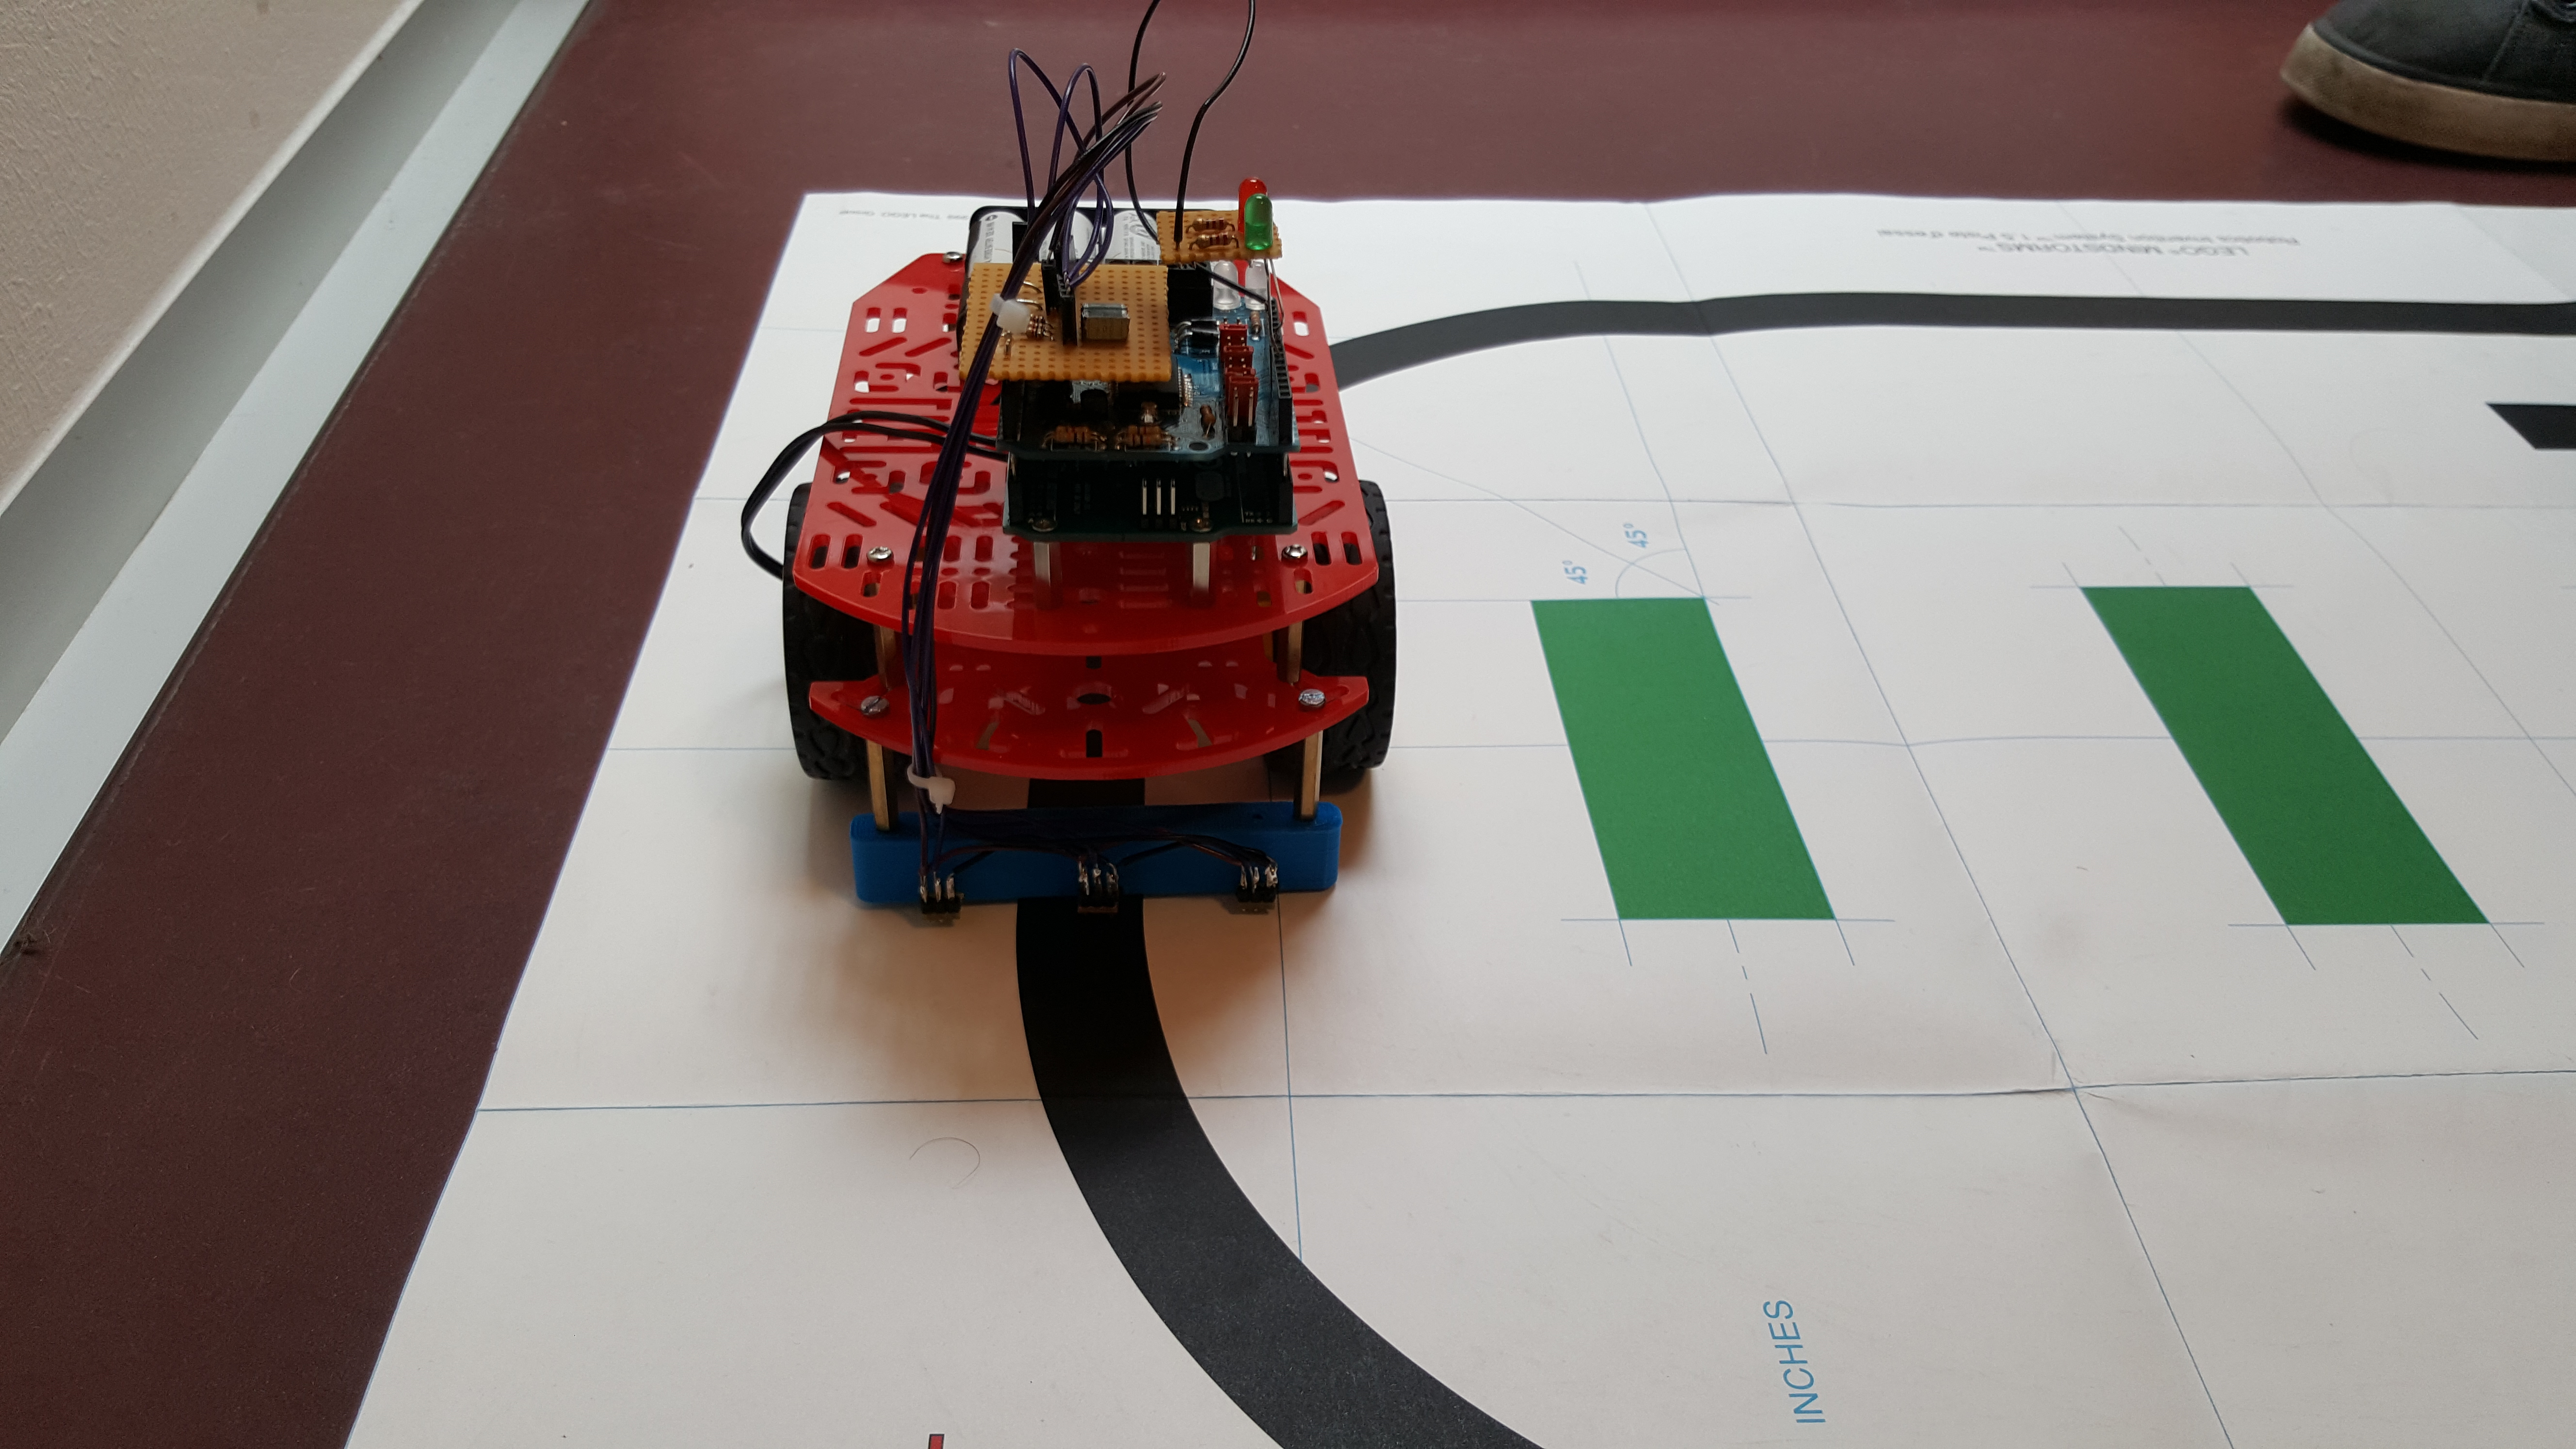
\includegraphics[width=0.6\textwidth]{figures/test3sensore.png}
  \caption{Test af Arduino kode med tre anvedte sensore.}
  \label{test_3_sensore}
\end{figure}




